\section{Results}
\label{sec:results}

\subsection{Language agents show inconsistent behavior over lifelong social interactions}
\label{sec:results:rq1}
\begin{figure}[!t]
    \centering
    
\includegraphics[width=0.92\textwidth]{figures/main/bel_goal_combined.pdf}
    
    \caption{Performance of language agents and humans across multiple episodes. (Left) Evolution of \believability scores with an increasing number of episodes. (Right) Evolution of \goalcompletion scores. Scores of all models decline for both dimensions with the simpler memory method, while the advanced memory method leads to significant improvement. Humans consistently demonstrate excellent performance.}
    \label{fig:main}
\end{figure}
\textbf{Performance of language agents with the entire interaction as memory} \quad Figure~\ref{fig:main} illustrates the performance of various language agents on the \believabilityFull dimension as the number of episodes increase. When provided with their complete interactions in an episode as memory, the performance of all the LLM-based agents shows a consistent decline on \believability. GPT-4o shows the most pronounced decline, with a steep drop in performance over the first few episodes. The decline is less severe for Gemini-1.5 and Llama-3.1, but still appreciable. A qualitative analysis of these episodes also reveals that the models increasingly fail on the 8 checkpoints within the \believabilityextended dimension. This directly results in the continuously decreasing \believability scores and also points to the fact that the \textbf{models become inconsistent over lifelong interactions.} The increased context length and information seem to overwhelm the agents, causing them to lose focus from the ongoing interaction and sometimes respond with utterances completely unrelated to the current conversation. This reduces the believability of conversations significantly as the number of episodes increase. Examples of some failure cases are provided in Appendix \S \ref{appendix:qual_belext}.

\subsection{Language agents are lacking in social intelligence}
\label{sec:results:rq2} 
\textbf{Performance of language agents with the entire interaction as memory} \quad Figure~\ref{fig:main} again shows the performance of the agents on \goalcompletionFull. We observe a similar trend as in \S \ref{sec:results:rq1}, where the performance of all LLMs declines with time. GPT-4o is once again the worst-performing model, followed by Llama-3.1 and Gemini-1.5. This suggests that \textbf{providing additional information to the agents has a detrimental effect on their performance.} Furthermore, decreasing consistency causes the agents not only to confuse their identities with those of other agents but also their current social goals with those from past scenarios, resulting in failures at goal completion in the current scenario. The inability of the models to learn from past interactions and adapt their strategies indicates a severe \textit{lack of social intelligence} and an inability to effectively plan for future interactions in dynamic, ever-changing goal settings.

\textbf{Human Performance in \lifelongsotopia} \quad To establish a baseline, we conducted the same experiments with humans interacting in the same setting. As shown in Figure \ref{fig:main}, humans display excellent scores across both \believability and \goalcompletion dimensions and maintain their performance throughout the interactions, \textbf{demonstrating consistency and exceptional goal completion ability.} While their numerical scores stay stable throughout and do not show an increase, a qualitative analysis of the episodes reveals that humans effectively use their past interactions to better plan and achieve their goals in subsequent scenarios. We observed instances where they adopt negotiation strategies from the other characters in the environment, learn about their behaviours and preferences, and leverage knowledge gained in previous episodes to optimize their goals in the current one. Please refer to Appendix \S \ref{appendix:qual:human} for more information on how humans use their past interactions to achieve their goals.

\subsection{An advanced memory module improves model performance, but they still show declining goal completion ability on harder scenarios}
\label{sec:results:rq3}
\textbf{Performance of language agents with an advanced memory module} \quad In Figure \ref{fig:main}, we also represent the performance of the language agents when equipped with an advanced memory module (as described in \S \ref{sec:framework:implementation}). \textbf{In this case, the performance of the agents improves significantly compared to the original setup.} Although Llama-3.1 still exhibits a decline in both \believability and \goalcompletion, the degradation in performance is much less severe than in the original case. In contrast, both GPT-4o and Gemini-1.5 demonstrate consistent performance across both dimensions, achieving near-perfect scores throughout. This indicates that equipping these agents with an advanced memory improves both their consistency and goal completion abilities.

\textbf{Hand-crafting harder social scenarios} \quad One limitation the way our previous episode chains are constructed is that the scenarios were generated independently while constructing the dataset. This combined with the random shuffling of episodes while chaining them together meant that the past context provided to them may not always be needed and approaching each scenario independently can also allow you to achieve near-perfect performance. Thus, to further investigate whether language agents equipped with the second type of memory are as good as humans, we \textbf{hand-craft 5 scenarios} which would explicitly require the language agents to make use of the context gained in their past interactions. Some of them directly relate to past scenarios and can also be follow up events to them requiring the agents to retrieve those memories or refer to them, while others may require negotiation strategies learnt previously or past knowledge gained to achieve their goals. Appendix \S \ref{appendix:hard_scenarios:details} gives details on the designed scenarios.

\textbf{Evaluating the Language Agents on Harder Scenarios} \quad Figure \ref{fig:hard} compares the performance of Gemini-1.5, GPT-4o, \review{Llama-3.1 and Llama-3.2} using the advanced memory module, alongside human performance, on simpler (left side of the black line) and harder, hand-crafted scenarios (right side of the black line) across both the \believability and \goalcompletion dimensions. The \believability scores remain consistent, indicating that the language agents are able to maintain character consistency in both simple and complex scenarios. However, the interesting trend lies in their performance on \goalcompletion. \textbf{While humans maintain their goal completion abilities even in the harder scenarios, the performance of \review{all the LLM-based models equipped with the advanced memory module} declines sharply as soon as the harder scenarios begin}, where they are required to explicitly access and reason over their memory. A qualitative analysis of the interactions reveals similar findings: humans effectively leverage their past memories to accomplish their goals (Appendix \S \ref{appendix:hard_scenarios:humans}), while the language agents fail to show the same level of competence. This highlights the current limitations in social intelligence exhibited by these LLM-based agents and demonstrates that our benchmark, \lifelongsotopia, is an effective framework for identifying their shortcomings.
\begin{figure}[!t]
    \centering
    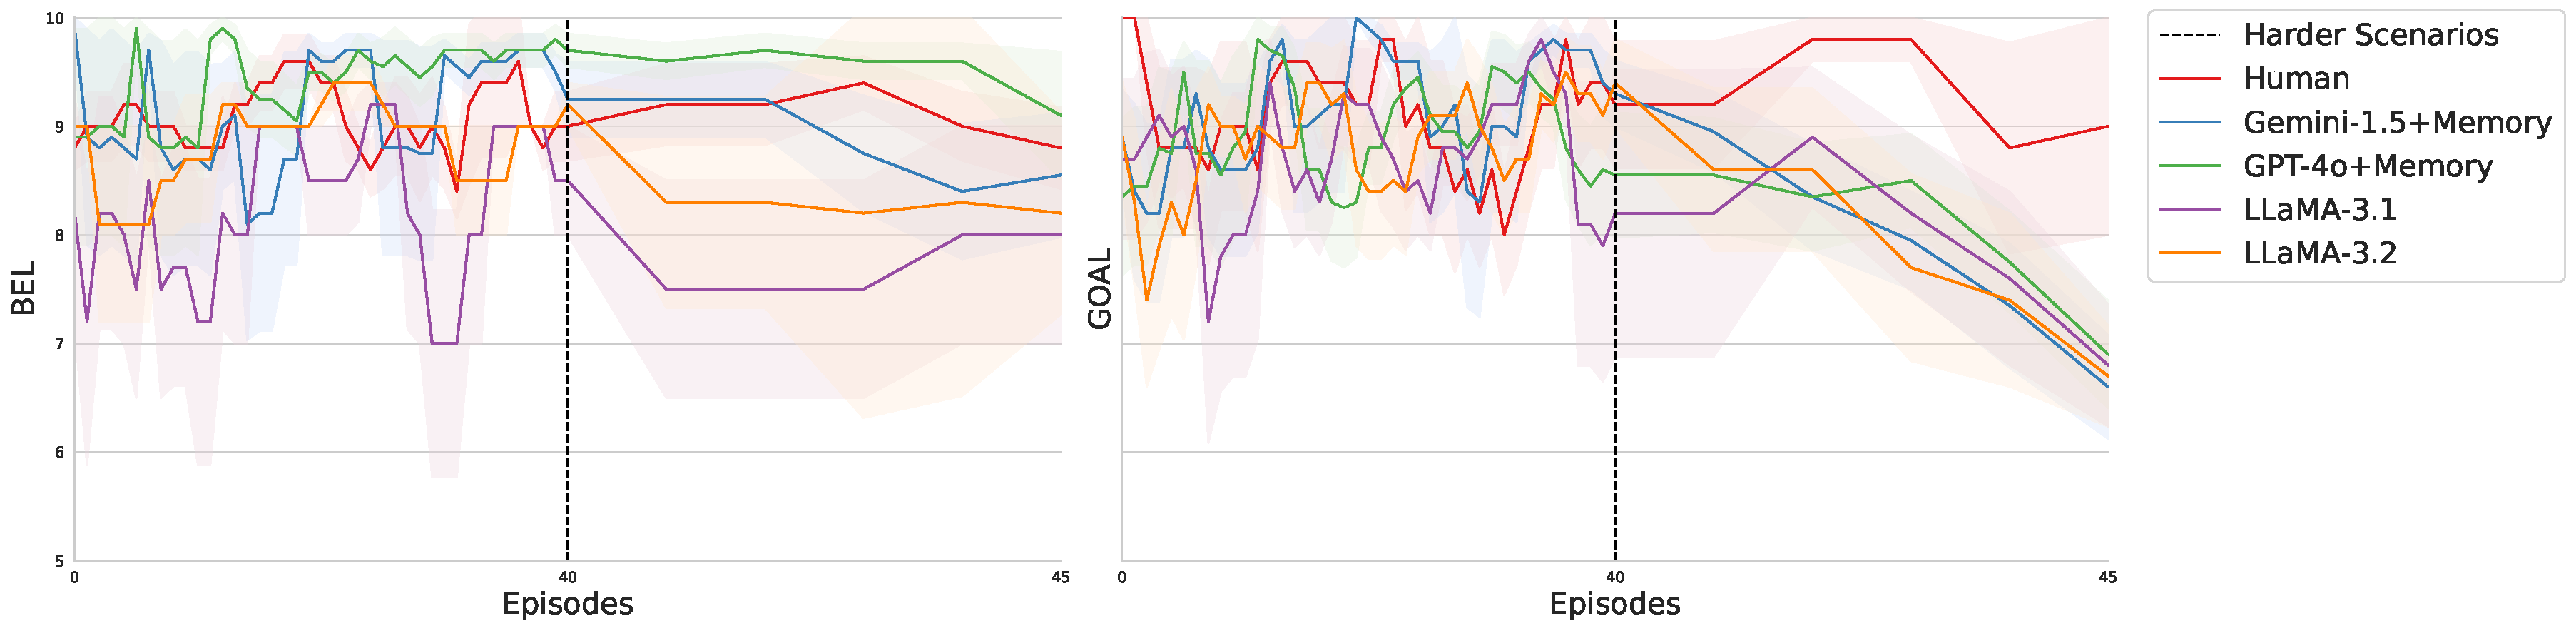
\includegraphics[width=0.92\textwidth]{figures/hard/bel_goal_combined.pdf}
    \caption{Performance of humans and language agents equipped with the advanced memory method upon the introduction of harder social scenarios. The black vertical line marks the beginning of the harder scenarios. (Left) \believability scores over increasing episodes. (Right) \goalcompletion scores. The models maintain their performance on \believability despite the harder scenarios, but their \goalcompletion scores drop significantly, unlike humans who maintain consistent performance.}
    \label{fig:hard}
\end{figure}
